\documentclass{article}

\usepackage[utf8]{inputenc}
\usepackage{hyperref}
\usepackage{xcolor}
\usepackage{graphicx}


\title{Le petit guide du mage noir}
\author{Joris Masson}
\date{\today}

\begin{document}

\maketitle
Voici Le petit guide du mage noir, qui sert à installer un serveur privé pour un certain jeu animé. Regardez le sommaire en dessous pour mieux vous y retrouver.
\tableofcontents

\newpage

\section{Pré-requis}
Pour commencer, il vous faudra, peu importe la version de Grasscutter que vous comptez installer, quelques pré-requis:
\begin{itemize}
	\item Java 17
	\item MongoDB
	\item Un proxy
\end{itemize}

\subsection{Java 17}
Pour java 17, c'est assez simple, allez \href{https://download.oracle.com/java/17/archive/jdk-17.0.3.1_windows-x64_bin.exe}{\textcolor{blue}{ici}}(téléchargement officiel).\newline
Une fois Java 17 installé, il vous faudra configurer votre variable JAVA\_HOME dans les variables d'environnement. Cherchez "variables d'environnement" sous Windows et vous devriez trouver.

\begin{figure}[!h]
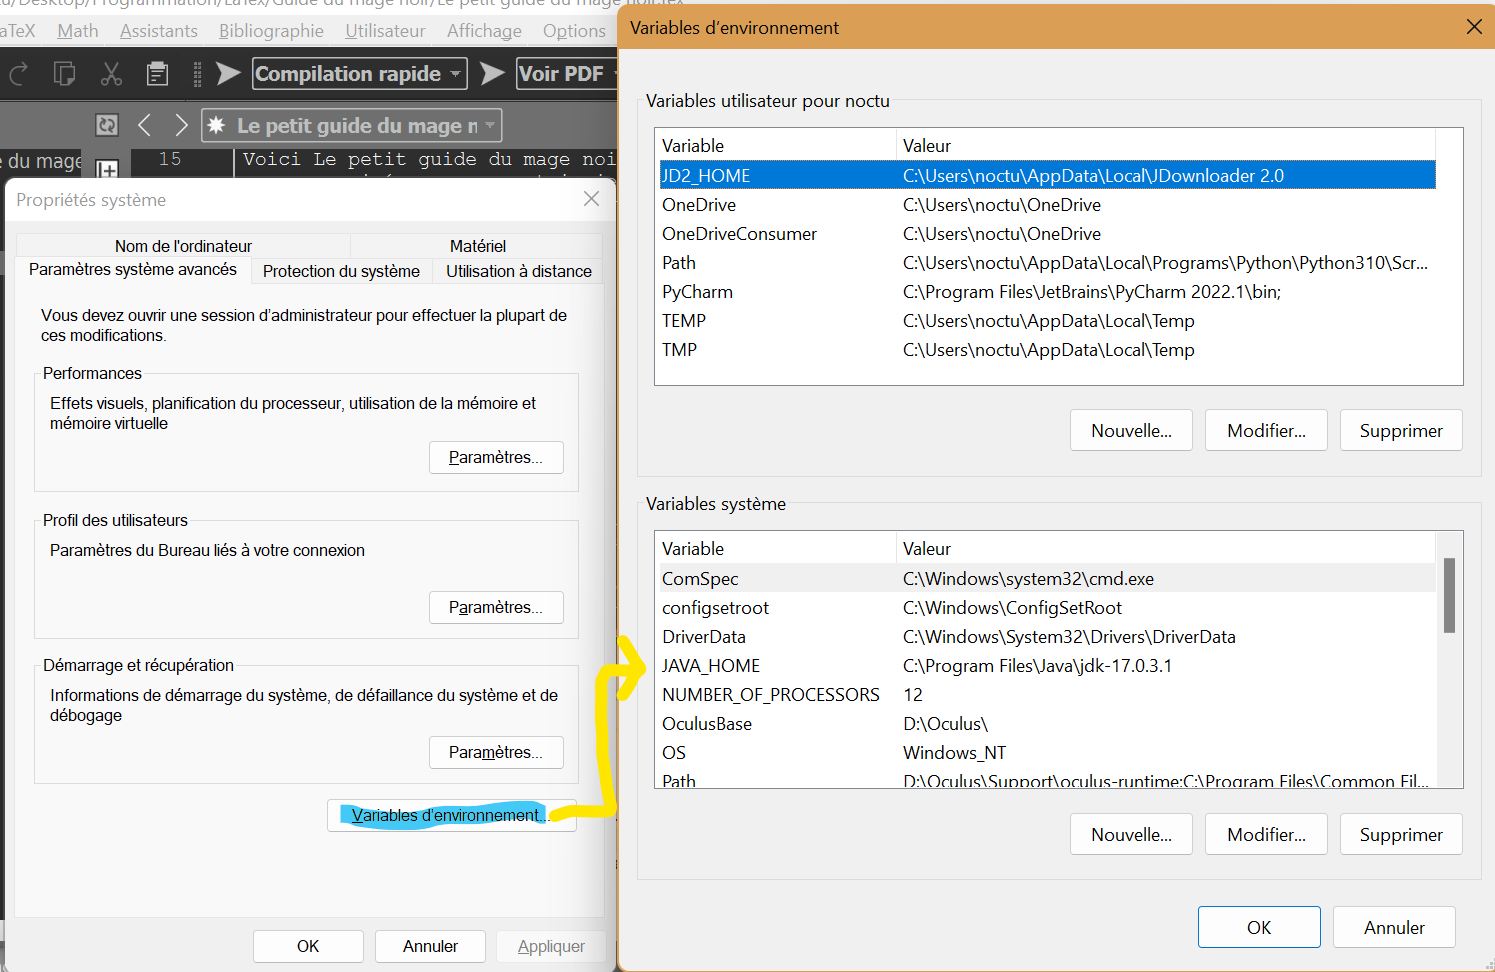
\includegraphics[scale=0.5]{img/env_var.png}
\end{figure}

Une fois que vous avez trouvé la bonne variable(si elle n'y est pas, vous pouvez la créer en cliquant sur "Nouvelle..."), changez sa valeur au dossier d'installation de votre java 17. Par défaut il est dans Programmes/Java, mais si vous avez changer son dossier d'installation, mettez ce chemin dans la variable. Il est possible qu'un redémarrage soit nécessaire pour que le changement soit actif.

\subsection{MongoDB}
Maintenant que java est installé et configuré, on passe à MongoDB.\newline
MongoDB vous servira à gérer la base de données de votre serveur, vous pourrez vous servir de MongoDB Compass pour y accéder et la modifier.\newline
\href{https://fastdl.mongodb.org/windows/mongodb-windows-x86_64-5.0.7-signed.msi}{\textcolor{blue}{Le lien de MongoDB}}\newline
Lors de l'installation, il vous faudra vous assurer que MongoDB est bien installé en temps que service. Si vous ne le faites pas, il est possible que vous ayez des difficultés plus tard. Accessoirement, si l'on vous propose d'installer MongoDB Compass, dites oui, c'est toujours utile.

\subsection{Le proxy}
Pour le proxy, vous avez deux solutions:
\begin{itemize}
	\item Fiddler
	\item Mitmproxy
\end{itemize}
Personnellement je vous recommande mitmproxy car il se lancera automatiquement lors du lancement du serveur, alors que Fiddler devra être lancé à la main à chaque fois.

\subsubsection{Fiddler}
Si vous choisissez d'utiliser Fiddler, il vous faudra \href{https://www.telerik.com/download/fiddler/fiddler4}{\textcolor{blue}{télécharger Fiddler classic.}}\newline
Une fois l'installation faite, allez dans tools puis HTTPS et cochez "Capture HTTPS CONNECTs" ainsi que "Decrypt HTTPS traffic"\newline
Puis, toujours dans les options allez dans connections et changez "Fiddler Classic listens on port" à autre chose que 8888.\newline
Ensuite fermez les options et sur la page principale, là où il y a vraiment beaucoup d'onglets, cliquez sur FiddlerScript et remplacez tout le script déjà présent par \href{https://github.lunatic.moe/fiddlerscript}{\textcolor{blue}{celui-ci}} et cliquez sur "Save Script".\newline
Fiddler est maintenant configuré!

\subsubsection{Mitmproxy}
Pour Mitmproxy il n'y a rien à faire si vous pensez utiliser Grassclipper. 

\section{Installation de Grasscutter}

\subsection{Version normale}

\subsection{Version beta(2.7)}

\section{Lancement du serveur}

\subsection{Lancement via CMD}

\subsection{Lancement via Grassclipper}


\end{document}
